\documentclass[tikz,border=10pt]{standalone}
\usepackage{tikz}
\usetikzlibrary{arrows.meta}

\begin{document}
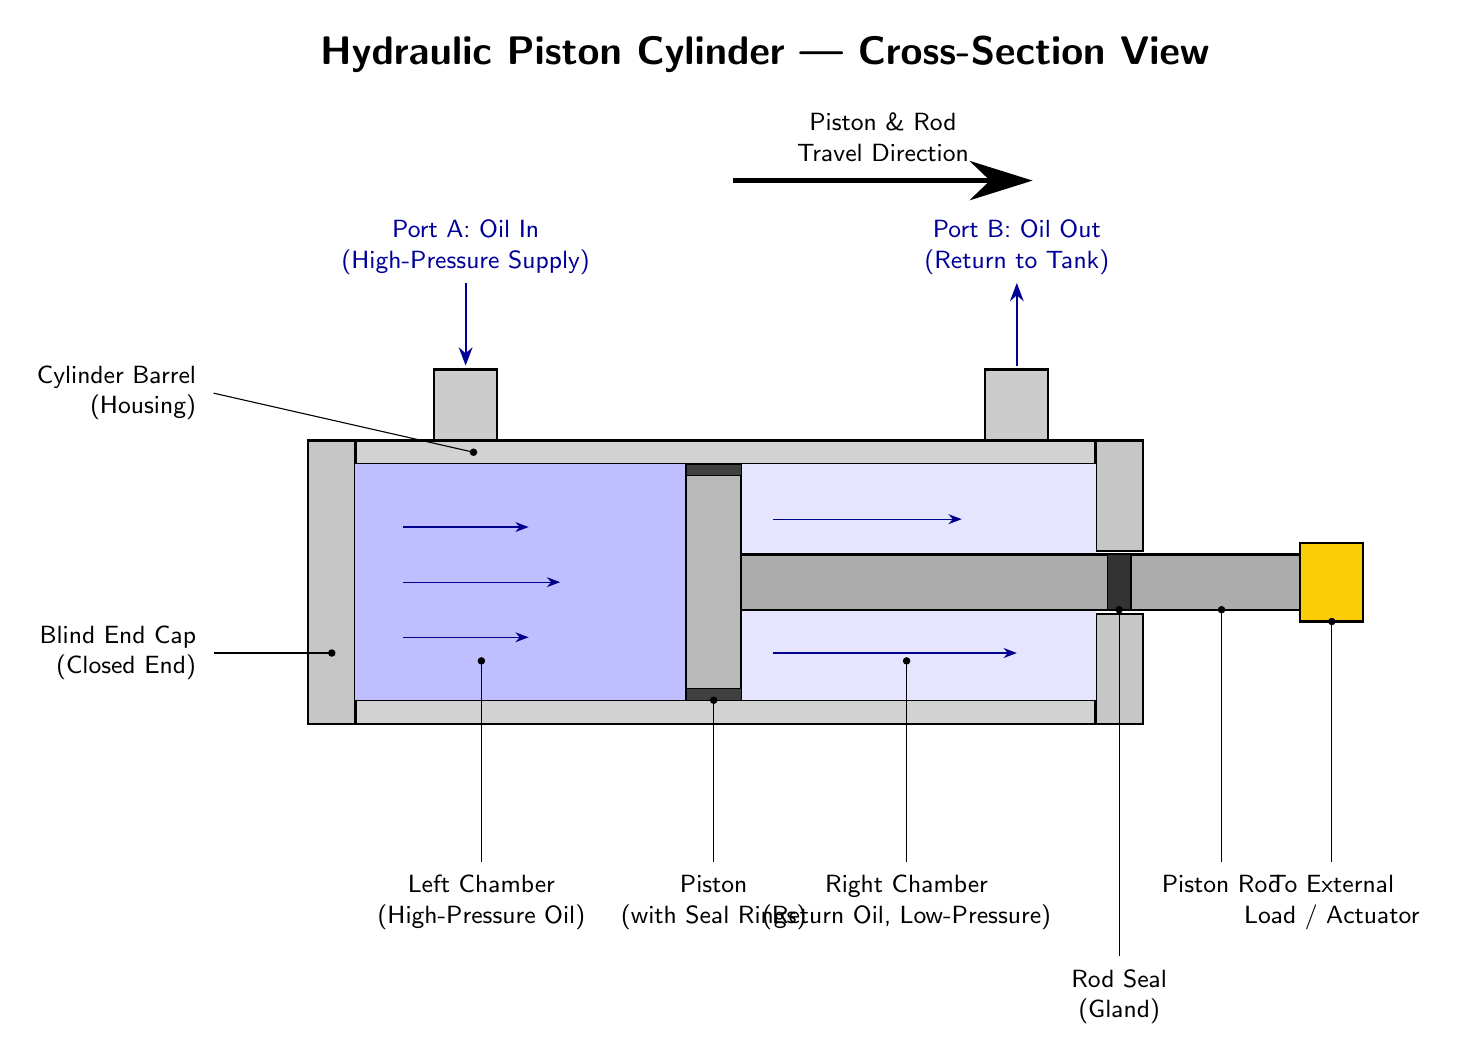
\begin{tikzpicture}[
  every node/.style={font=\sffamily\small},
  >=Stealth
]

% ---------- Title ----------
\node[font=\sffamily\Large\bfseries] at (6.2,9.2) {Hydraulic Piston Cylinder --- Cross-Section View};

% ---------- Piston / Rod motion arrow ----------
\draw[-{Stealth[length=8mm,width=5mm]}, ultra thick] (5.8,7.6) -- (9.6,7.6);
\node[align=center] at (7.7,8.15) {Piston \& Rod\\Travel Direction};

% ---------- Port A (inlet, blind end) ----------
\filldraw[fill=gray!40, draw=black, thick] (2.0,4.3) rectangle (2.8,5.2);
\draw[->, thick, blue!60!black] (2.4,6.3) -- (2.4,5.25);
\node[align=center, text=blue!60!black] at (2.4,6.75) {Port A: Oil In\\(High-Pressure Supply)};

% ---------- Port B (outlet, rod end) ----------
\filldraw[fill=gray!40, draw=black, thick] (9.0,4.3) rectangle (9.8,5.2);
\draw[->, thick, blue!60!black] (9.4,5.25) -- (9.4,6.3);
\node[align=center, text=blue!60!black] at (9.4,6.75) {Port B: Oil Out\\(Return to Tank)};

% ---------- Cylinder outer walls ----------
\filldraw[fill=gray!35, draw=black, thick] (1.0,4.0) rectangle (10.4,4.3); % top wall
\filldraw[fill=gray!35, draw=black, thick] (1.0,0.7) rectangle (10.4,1.0); % bottom wall

% ---------- End caps ----------
\filldraw[fill=gray!45, draw=black, thick] (0.4,0.7) rectangle (1.0,4.3); % blind end cap
\filldraw[fill=gray!45, draw=black, thick] (10.4,2.90) rectangle (11.0,4.3); % rod end cap - top segment
\filldraw[fill=gray!45, draw=black, thick] (10.4,0.7) rectangle (11.0,2.10); % rod end cap - bottom segment

% ---------- Chambers (hydraulic fluid) ----------
\filldraw[fill=blue!25, draw=none] (1.0,1.0) rectangle (5.2,4.0); % left / blind-end chamber
\filldraw[fill=blue!10, draw=none] (5.9,2.85) rectangle (10.4,4.0); % right chamber - upper lobe
\filldraw[fill=blue!10, draw=none] (5.9,1.0) rectangle (10.4,2.15); % right chamber - lower lobe

% ---------- Flow arrows inside chambers ----------
\draw[->, blue!55!black] (1.6,3.2) -- (3.2,3.2);
\draw[->, blue!55!black] (1.6,2.5) -- (3.6,2.5);
\draw[->, blue!55!black] (1.6,1.8) -- (3.2,1.8);

\draw[->, blue!55!black] (6.3,3.3) -- (8.7,3.3);
\draw[->, blue!55!black] (6.3,1.6) -- (9.4,1.6);

% ---------- Piston ----------
\filldraw[fill=gray!55, draw=black, thick] (5.2,1.0) rectangle (5.9,4.0);
\filldraw[fill=black!75, draw=black] (5.2,3.85) rectangle (5.9,4.0); % top seal ring
\filldraw[fill=black!75, draw=black] (5.2,1.0) rectangle (5.9,1.15); % bottom seal ring

% ---------- Rod ----------
\filldraw[fill=gray!65, draw=black, thick] (5.9,2.15) rectangle (13.0,2.85);
\filldraw[fill=black!80, draw=black] (10.55,2.15) rectangle (10.85,2.85); % rod gland seal

% ---------- Load block ----------
\filldraw[fill=yellow!65!orange, draw=black, thick] (13.0,2.0) rectangle (13.8,3.0);

% ---------- Side labels: cylinder barrel & blind end cap ----------
\draw[thin] (-0.8,4.9) -- (2.5,4.15);
\filldraw (2.5,4.15) circle (0.04);
\node[align=right, anchor=east] at (-0.9,4.9) {Cylinder Barrel\\(Housing)};

\draw[thin] (-0.8,1.6) -- (0.7,1.6);
\filldraw (0.7,1.6) circle (0.04);
\node[align=right, anchor=east] at (-0.9,1.6) {Blind End Cap\\(Closed End)};

% ---------- Bottom labels ----------
\draw[thin] (2.6,1.5) -- (2.6,-1.05);
\filldraw (2.6,1.5) circle (0.04);
\node[align=center, anchor=north] at (2.6,-1.1) {Left Chamber\\(High-Pressure Oil)};

\draw[thin] (5.55,1.0) -- (5.55,-1.05);
\filldraw (5.55,1.0) circle (0.04);
\node[align=center, anchor=north] at (5.55,-1.1) {Piston\\(with Seal Rings)};

\draw[thin] (8.0,1.5) -- (8.0,-1.05);
\filldraw (8.0,1.5) circle (0.04);
\node[align=center, anchor=north] at (8.0,-1.1) {Right Chamber\\(Return Oil, Low-Pressure)};

\draw[thin] (12.0,2.15) -- (12.0,-1.05);
\filldraw (12.0,2.15) circle (0.04);
\node[align=center, anchor=north] at (12.0,-1.1) {Piston Rod};

\draw[thin] (13.4,2.0) -- (13.4,-1.05);
\filldraw (13.4,2.0) circle (0.04);
\node[align=center, anchor=north] at (13.4,-1.1) {To External\\Load / Actuator};

\draw[thin] (10.7,2.15) -- (10.7,-2.25);
\filldraw (10.7,2.15) circle (0.04);
\node[align=center, anchor=north] at (10.7,-2.3) {Rod Seal\\(Gland)};

\end{tikzpicture}
\end{document}
